\chapter{Support Vector Machines}
In this chapter, we will explore what are known as support vector machines, or SVMs for short. SVMs are broadly useful for problems in classification and regression, and they are part of a family of techniques known as \textit{margin methods}. The defining goal of margin methods, and SVMs specifically, is to put as much distance as possible between data points and decision boundaries. We will dig deeper into what exactly this means over the course of the chapter. One of the most appealing aspects of SVMs is that they can be solved as convex optimization problems, for which we can find a global optimum with relative ease. We will explore the mathematical underpinnings of SVMs, which can be slightly more challenging than our previous topics, as well as their typical use cases.

\section{Motivation}
While SVMs can be used for classification or regression, we will reason about them in the classification case as it is more straightforward. 

The grand idea behind SVMs is that we should construct a linear hyperplane in our feature space that maximally separates our classes, which means that the different classes should be as far from that hyperplane as possible. The distance of our data from the hyperplane is known as \textit{margin}.

\begin{definition}{Margin}{definition}
Margin is the distance of the nearest data point from the separating hyperplane of an SVM model, as seen in Figure \ref{fig:2d-hyperplane}. Larger margins often lead to more generalizable models.
\end{definition}

A larger margin tends to mean that our model will generalize better, since it provides more wiggle room to correctly classify unseen data (think about new data being a perturbation on current data).

\begin{figure}
    \centering
    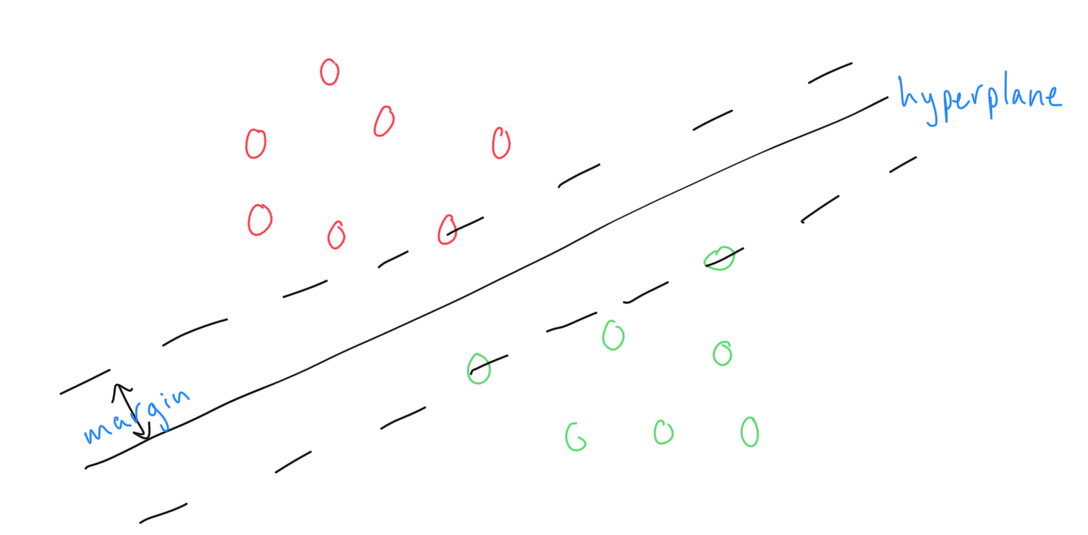
\includegraphics[width=0.5\paperwidth]{../SupportVectorMachines/fig/2d-hyperplane.png}
    \caption{Hyperplane with margin between different classes.}
    \label{fig:2d-hyperplane}
\end{figure}

This idea of the margin of a separator is quite intuitive. If you were presented with Figure \ref{fig:2d-hyperplane} and were asked to separate the two classes, you would likely draw the line that keeps data points as far from it as possible. SVMs and other margin-based methods will attempt to algorithmically recreate this intuition.

\subsection{Max Margin Methods}
SVMs are a specific instance of a broader class of model known as \textit{max margin methods}. Their name describes them well: they deal with creating a maximum margin between training data and decision boundary, with the idea that this leads to model generalizability. 

Other max margin methods are outside the scope of this textbook. These alternative methods may differ from SVMs in a non-trivial way. For example, SVMs do not produce probabilities  on different classes, but rather decision rules for handling new data points. If you needed probabilities, there are other max margin methods that can be used for the task.
%
\begin{mlcube}{Support Vector Machines}
SVMs are typically used in settings with discrete outputs. We need labeled training data to identify the relevant hyperplane in an SVM model. Finally, SVMs operate in a non-probabilistic setting.
\begin{center}
    \begin{tabular}{c|c|c}
    \textit{\textbf{Domain}} & \textit{\textbf{Training}} & \textit{\textbf{Probabilistic}} \\
    \hline
    Discrete & Supervised & No \\
    \end{tabular}
\end{center}
\end{mlcube}

\subsection{Applications}
The theory behind SVMs has been around for quite some time (since 1963), and prior to the rise of neural networks and other more computationally intensive techniques, SVMs were used extensively for image recognition, object categorization, and other typical machine learning tasks.

SVMs are still widely used in practice, for example for  classification problems known as anomaly detection.
%
\readernote{The purpose of anomaly detection is to identify unusual data points. For example, if we are manufacturing shoes, we may wish to inspect and flag any shoe that seems atypical with respect to the rest of the shoes we produce.}

Anomaly detection can be as simple as a binary classification problem where the data set is comprised of anomalous and non-anomalous data points. As we will see, an SVM can be constructed from this data set to identify future anomalous points very efficiently. SVMs extend beautifully to settings where we want to use basis functions, and thus non-linear interactions on features. For this reason, they continue to be competitive in many real-world situations where these kinds of interactions are important to work with.

\section{Hard Margin Classifier for Linearly Separable Data}

We will learn the theory behind SVMs by starting with a simple two-class classification problem, as we've seen several times in previous chapters. We will constrain the problem even further by assuming, at least to get started, that the two classes are linearly separable, which is the basis of the \textit{hard margin} formulation for SVMs.

\readernote{The expression `hard margin' simply means that we don't allow any data to be classified incorrectly. If it's not possible to find a hyperplane that perfectly separates the data based on class, then the hard margin classifier will return no solution.}

\subsection{Why the Hard Margin}
The hard margin constraint, which assumes that our data is linearly separable, is not actually a requirement for constructing an SVM, but it simplifies the problem initially and makes our derivations significantly easier. After we've established the hard margin formulation, we will extend the technique to work in situations where our data is not linearly separable.

\subsection{Deriving our Optimization Problem}
Recall that our goal is to define a hyperplane that separates our data points and maintains the maximum possible distance between the hyperplane and nearest data points on either side of it.
There are  $N$ examples  $\textbf{x}_{1}, ..., \textbf{x}_{N}$ and there is a bias term $w_{0}$.
Each example has a label $y_{1}, ..., y_{N}$ which is either $1$ or $-1$. 
To uncover this hyperplane, we start with a simple linear model for a two-class classification problem:
\begin{equation} \label{classification-fn}
h(\textbf{x}) = \textbf{w}^\top \textbf{x} + w_{0}.
\end{equation}

This is the {\em discriminant function} and we classify a new example to class $1$ or $-1$ according to the sign produced by our trained model $h(\textbf{x})$. Later, we will also make this more general by using a basis function, 
$\phi(\mathbf{x})$ to transform to a higher dimensional feature space.

By specifying our model this way, we have implicity defined a hyperplane separating our two classes given by:
\begin{equation} \label{implicit-hyperplane}
	\textbf{w}^\top \textbf{x} + w_{0} = 0
\end{equation}
Furthermore, we have that $\textbf{w}$ is orthogonal to the hyperplane, which we demonstrate now:

\begin{derivation}{Hyperplane Orthogonal to $\textbf{w}$}{hyperplane-derivation}
	Imagine two data points $\mathbf{x}_{1}$ and $\mathbf{x}_{2}$ on the hyperplane defined by $\textbf{w}^\top \textbf{x} + w_{0} = 0$. When we project their difference onto our model $\textbf{w}$, we find:
	\begin{equation} \label{hyperplane-eqn}
		\textbf{w}^\top(\textbf{x}_{1} - \textbf{x}_{2}) = \textbf{w}^\top\textbf{x}_{1} - \textbf{w}^\top\textbf{x}_{2} = -w_{0} - (-w_{0}) = 0
	\end{equation}
	which means that $\textbf{w}$ is orthogonal to our hyperplane. We can visualize this in Figure \ref{fig:orthogonal-w}.
\end{derivation}

\begin{figure}
    \centering
    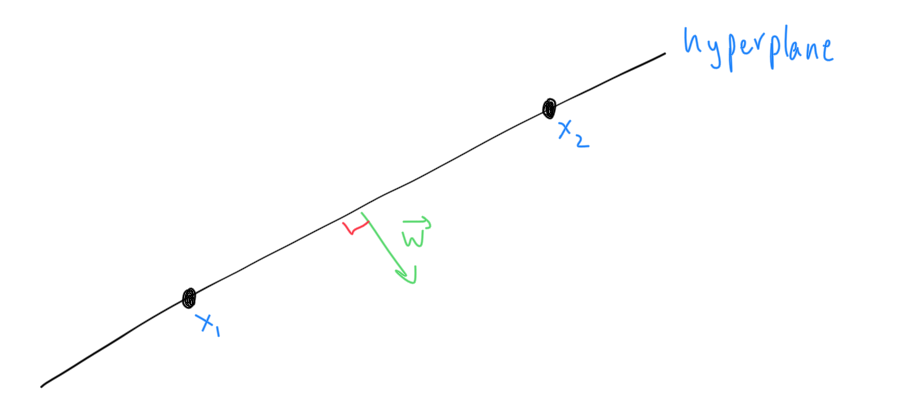
\includegraphics[width=0.5\paperwidth]{../SupportVectorMachines/fig/orthogonal-w.png}
    \caption{Our weight vector \textbf{w} is orthogonal to the separating hyperplane.}
    \label{fig:orthogonal-w}
\end{figure}

Remember that we're trying to maximize the margin between our training data and the hyperplane. The fact that $\textbf{w}$ is orthogonal to our hyperplane will help with this.

To determine the distance between a data point $\textbf{x}$ and the hyperplane, which we denote $d$, we need the distance in the direction of $\textbf{w}$ between the point and the hyperplane. We denote $\textbf{x}_{p}$ to be the projection of $\textbf{x}$ onto the hyperplane, which allows us to decompose $\textbf{x}$ as the following:
\begin{equation} \label{decompose-x}
	\textbf{x} = \textbf{x}_{p} + d \frac{\textbf{w}}{|| \textbf{w} ||_2}
\end{equation}
which is the sum of the portion of the projection of $\textbf{x}$ onto the hyperplane and the portion of $\textbf{x}$ that is parallel to $\textbf{w}$ (and orthogonal to the hyperplane). From here we can solve for $d$:
%
\begin{derivation}{Distance from Hyperplane Derivation}{distance-from-hyperplane-derivation}
	We start by left multiplying Equation \ref{decompose-x} with $\textbf{w}^\top$,
	\begin{align*}
		\textbf{w}^\top\textbf{x} = \textbf{w}^\top\textbf{x}_{p} + d \frac{\textbf{w}^\top\textbf{w}}{||\textbf{w}||_2}.
	\end{align*}
	Simplifying (note that $\textbf{w}^\top\textbf{x}_{p} = -w_{0}$ from Equation \ref{hyperplane-eqn}):
	\begin{align*}
		\textbf{w}^\top\textbf{x} =  - w_{0} + d ||\textbf{w}||_2
	\end{align*}
	Rearranging:
	\begin{align*}
		d = \frac{\textbf{w}^\top\textbf{x} + w_{0}}{||\textbf{w}||_2}.
	\end{align*}
\end{derivation}

For each data point $\textbf{x}$, we now have the signed distance of that data point from the hyperplane.

For an example that is classified correctly, this signed distance $d$ will be positive for class $y_n = 1$, and negative for class $y_n = -1$.  Given this, we can make the distance unsigned (and always   positive) for a correctly classified data point by multiplying by $y_n$. Then, the {\em margin for an correctly classified data point $(\textbf{x}_{n},y_n)$} is given by:
\begin{equation} \label{individual-margin}
	\frac{y_{n}(\textbf{w}^\top\textbf{x}_{n} + w_{0})}{||\textbf{w}||_2}.
      \end{equation}
      
      The margin for an entire data set is given by the margin to the closest point in the data set,  and
      %
\begin{equation} \label{total-margin}
	\min_{n} \frac{y_{n}(\textbf{w}^\top\textbf{x}_{n} + w_{0})}{||\textbf{w}||_2}.
\end{equation}

Then, it is our goal to maximize this margin with respect to our model parameters $\textbf{w}$ and $w_{0}$. This is given by:
\begin{equation} \label{total-maximized-margin}
  \underset{\textbf{w}, w_{0}}{\max}  \ \ \frac{1}{||\textbf{w}||_2} \left[\min_{n} y_{n}(\textbf{w}^\top\textbf{x}_{n} + w_{0}) \right]
\end{equation}

Here, we pull the $1/||\mathbf{w}||_2$ term forward. Note carefully that $w_0$ does not play a role in the denominator $||\mathbf{w}||_2$.

This is a hard problem to optimize, but we can make it more tractable by recognizing some important features of Equation \ref{total-maximized-margin}. First, rescaling $\textbf{w} \rightarrow \alpha \textbf{w}$ and $w_{0} \rightarrow \alpha w_{0}$, for any $\alpha >0$, has no impact on the margin for any correctly classified data point $\textbf{x}_{n}$. This is because the effect of $\alpha$ cancels out in the numerator and denominator of Equation~\ref{individual-margin}.

We can use this rescaling liberty to enforce
%
\begin{equation} \label{new-margin-constraint}
  y_{n}(\textbf{w}^\top\textbf{x}_{n} + w_{0}) \geq 1,  \quad \quad \mbox{for all $n$}.
\end{equation}

This does not change the optimal margin because we can always scale up both $\mathbf{w}$ and $w_0$ by $\alpha>0$ to achieve
$ y_{n}(\textbf{w}^\top\textbf{x}_{n} + w_{0}) \geq 1$, and without affecting the margin. Moreover, since the problem is to maximize $1/||\mathbf{w}||_2$, an optimal solution will want $||\mathbf{w}||_2$ to be as small as possible, and thus at
least one of these constraints~\eqref{new-margin-constraint} will be binding and equal to one  in an optimal solution. 

Thus our optimization problem now looks like:
\begin{equation} \label{simplified-maximized-margin-optimization}
	\underset{\textbf{w}, w_{0}}{\max} \ \ \frac{1}{||\textbf{w}||_2} \quad \text{s.t.} \quad y_{n}(\textbf{w}^\top\textbf{x}_{n} + w_{0}) \geq 1, \quad \mbox{for all $n$}.
      \end{equation}

      Here, we recognized that $\min_{n} y_{n}(\textbf{w}^\top\textbf{x}_{n} + w_{0})=1$ in an optimal solution with these new constraints,
      and adopted this in the objective.  This simplifies considerably, removing the ``min $_n$'' part of the objective.
      
Notice that maximizing $\frac{1}{||\textbf{w}||_2}$ is equivalent to minimizing $||\textbf{w}||_2^{2}$. We will also add a constant term $\frac{1}{2}$ for convenience, leaving the {\bf hard-margin formulation of the training problem}:
%
\begin{equation} \label{final-simplified-maximized-margin-optimization}
	\underset{\textbf{w}, w_{0}}{\min}\ \  \frac{1}{2} ||\textbf{w}||_2^{2} \quad \text{s.t.} \quad y_{n}(\textbf{w}^\top\textbf{x}_{n} + w_{0}) \geq 1, \quad \mbox{for all $n$}.
\end{equation}

Note that Equation \ref{final-simplified-maximized-margin-optimization} is now a quadratic programming problem, which means we wish to optimize a quadratic function subject to a set of linear constraints on our parameters. Arriving at this form was the motivation for the preceding mathematic manipulations. We will discuss shortly how we actually optimize this function.

\subsection{What is a Support Vector}

Up until now, we have discussed Support Vector Machines without identifying what a support vector is. We now have enough information from the previous section to define them. Later, when we work with a dual formulation, we will see the precise role that they play.

Say that an
example is on the {\em margin boundary}
if $y_{n}(\textbf{w}^\top\textbf{x}_{n} + w_{0}) =1$. These are the points that are closest to the hyperplane and have margin $1/||{\mathbf w}||_2$.
%
\begin{definition}{Support Vector}{support-vector}
  A support vector in a  hard-margin SVM  formulation  must be a data point that is on
  the margin boundary of the optimal solution, with $y_{n}(\textbf{w}^\top\textbf{x}_{n} + w_{0}) =1$ and margin $1/||{\mathbf w}||_2$.
\end{definition}

In the hard margin case we have constrained the closest data points to
have discriminant value $\textbf{w}^\top\textbf{x}_{n} + w_{0} = 1$ ($-1$ for a negative example).
Figure \ref{fig:hard-margin-svm} shows a hard margin SVM solution with an illustration of
corresponding support vectors.

\readernote{After we have optimized an SVM in the hard margin case, we must have at least two support vectors with
  discriminant value that is 1 or -1, and thus a margin of $1/||\mathbf{w}||_2$.}

\readernote{Not every example on the margin boundary needs to be a support vector.}

\begin{figure}
    \centering
    \textbf{Hard Margin SVM Example}\par\medskip
    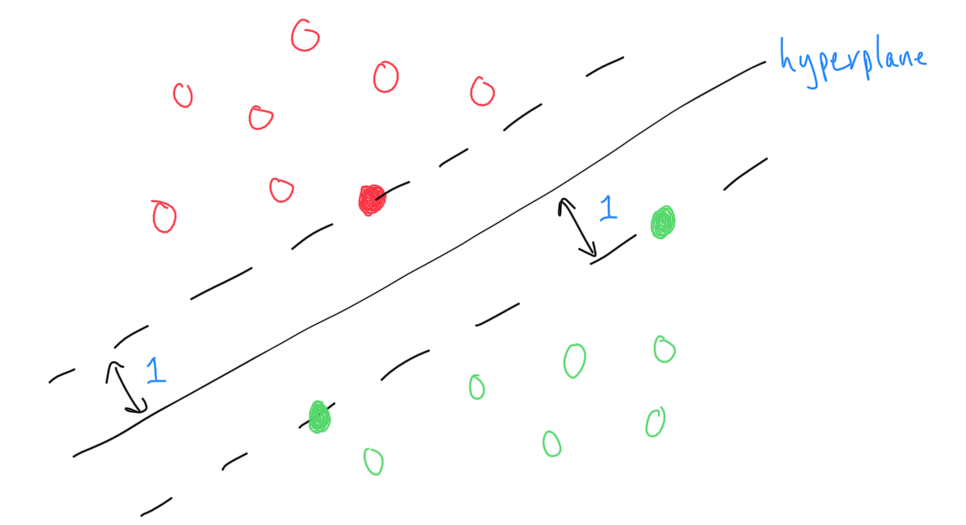
\includegraphics[width=0.5\paperwidth]{../SupportVectorMachines/fig/hard-margin-svm.png}
    \caption{Example of the resulting hyperplane for a hard margin SVM. The filled in data points are
      support vectors in this example. A support vector for the hard-margin formulation must be on the margin boundary, with a discriminant value of +1 or -1.}
    \label{fig:hard-margin-svm}
\end{figure}

\section{Soft Margin Classifier}

Thus far, we've been operating under the assumption that our data is linearly separable in feature space, which afforded us several convenient guarantees in the derivations of the previous section. For example, given that our data was linearly separable, we could guarantee that every data point would be on the correct side of the hyperplane, which waswhat allowed us to enforce the constraint that  $y_{n}(\textbf{w}^\top\textbf{x}_{n} + w_{0}) \geq  1$.
We now seek to generalize the work of the previous section to situations where our data is not
separable.

\subsection{Why the Soft Margin?}

What if our data is not linearly separable in the feature space (even after applying a basis function)?
This is the likely case in real applications!   Unfortunately, our current hard margin SVM formulation would be useless with non-linearly separable data. That is why we need the soft margin SVM.

\begin{figure}
    \centering
    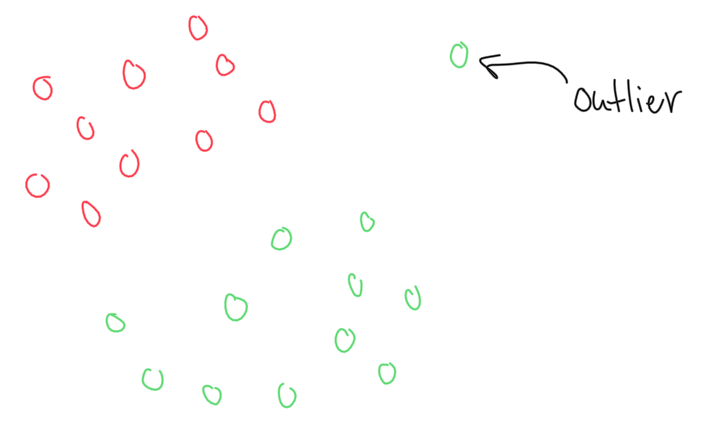
\includegraphics[width=0.5\paperwidth]{../SupportVectorMachines/fig/outlier-data-pt.png}
    \caption{An outlier can make the hard margin formulation impossible or unable to generalize well.}
    \label{fig:outlier-data-pt}
\end{figure}

At a high level, the soft margin SVM allows for some of our data points to be closer to or even on the incorrect side of the hyperplane. This is desirable if our data set is not linearly separable or contains outliers, and it is also quite intuitive. Examining Figure \ref{fig:outlier-data-pt}, we see that we have a single outlier data point. We can still create a good model by just allowing this single data point to be close to the hyperplane (or in some cases, even on the wrong side of the hyperplane). That is what the soft margin formulation will allow for.

\subsection{Updated Optimization Problem for Soft Margins}

To enable the soft margin formulation, we introduce what are known as \textit{slack variables} denoted $\xi_{n} \geq 0$, which simply relax the constraint from Equation \ref{simplified-maximized-margin-optimization} that we imposed in the hard margin formulation.
Say that a data point is ``inside the margin region'' if its discriminant value is in the range $(-1,+1)$.
%
There is a slack variable $\xi_{n} \geq 0$ for every data point $\textbf{x}_{n}$, and they take the following values according to how we classify $\textbf{x}_{n}$:
%
\begin{equation} \label{slack-variable-values}
	\xi_{n} = \begin{cases}
	 	= 0 & \text{if  $\textbf{x}_{n}$  is correctly classified} \\
		\in (0, 1] & \text{if $\textbf{x}_{n}$  is correctly classified but inside the  margin region} \\
		> 1 & \text{if $\textbf{x}_{n}$ is  incorrectly classified} \\
	\end{cases}
      \end{equation}
      
      These slack variable penalize data points on the wrong side of the margin boundary, but they don't forbid us from allowing data points to be on the wrong side if this produces the best model.
      We now reformulate the optimization problem as follows. This is the {\bf soft-margin training problem}:
%
%
      \begin{align} \label{soft-margin-optimization-problem}
  \underset{\textbf{w}, w_{0}, \bm \xi}{\min}\ &  \frac{1}{2} ||\textbf{w}||_2^{2} + C \sum_{n=1}^{N} \xi_{n}\\
  \mbox{s.t.}\quad & y_{n}(\textbf{w}^\top\textbf{x}_{n} + w_{0}) \geq 1 - \xi_{n}, \quad \mbox{for all $n$} \notag \\
  &\quad \xi_{n} \geq 0, \quad \mbox{for all $n$}. \notag
\end{align}

Here, $C$ is a regularization parameter that determines how heavily we penalize violations of the hard margin constraints. A large $C$ penalizes violation of the hard margin constraints more heavily, which means our model will follow the data closely and have small regularization. A small $C$ won't heavily penalize having data points inside the margin region, relaxing the constraint and allowing our model to somewhat disregard more of the data. This means more regularization.

\readernote{Unlike most regularization parameters we've seen thus far, $C$ increases regularization as it gets smaller.}

\subsection{Soft Margin Support Vectors}
Under the the hard margin formulation, the support vectors were some subset of the  data points with $y_{n}(\textbf{w}^\top\textbf{x}_{n} + w_{0})=1$,
and so situated exactly on the margin boundary,  and  they points
closest to the hyperplane.
%Under the soft margin formulation, we no longer have this guarantee since we explicity relaxed it in the name of creating better, more generalizable models.

The support vectors in the soft margin case must be data points that are either  on the margin boundary (and thus $y_{n}(\textbf{w}^\top\textbf{x}_{n} + w_{0})=1$) or for which $\xi_n\in (0,1]$ and in the margin region, or that are misclassified (when $\xi_{n} > 1$). We can visualize this in Figure \ref{fig:soft-margin-svm}.


\readernote{Not every data point on the margin boundary, in the margin region, or that is misclassified needs to be a support vector in the soft-margin
  formulation. But those that become support vectors must meet one of these criteria.}
%
\begin{figure}
    \centering
    \textbf{Soft Margin SVM Example}\par\medskip
    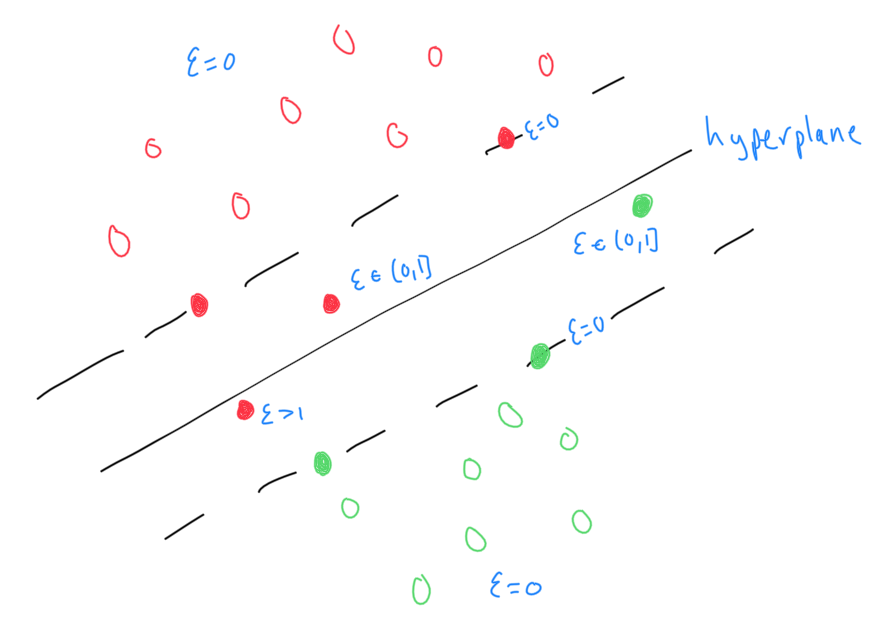
\includegraphics[width=0.5\paperwidth]{../SupportVectorMachines/fig/soft-margin-svm.png}
    \caption{Example of the resulting hyperplane for a soft margin SVM. The filled in data points illustrate the support vectors in this example and must be either on the margin boundary or on the ``wrong side'' of the margin boundary.}
    \label{fig:soft-margin-svm}
\end{figure}

\section{Conversion to Dual Form}

Now that we have the formulation of the optimization problem for SVMs, we need to discuss how we actually go about optimizing to produce a model solution. This will involve converting to a \textit{dual form} of our problem. We will do this in the hard margin case for technical simplicity, but our solution can be easily modified to also  apply to the soft margin formulation.

\readernote{A dual form is an equivalent manner of representing an optimization problem, in this case the quadratic programming problem we need to optimize. Dual forms can be easier to work with than their initial form (``the primal form.'')}

The dual form will be useful because it will allow us to bring in a basis function into the SVM formulation in a very elegant
and computationally efficient way.

\subsection{Lagrange Multipliers}

Before we get into deriving the dual form, we need to be aware of a critical piece of math that will enable us to solve our optimization problem: \textit{Langrange multipliers}.

A Lagrange multiplier is used to find optima of a function subject to certain constraints. This is exactly what we need to solve the optimization problem described by Equation \ref{final-simplified-maximized-margin-optimization}.

The underlying theory behind Lagrange multipliers is not overly difficult to understand, but it is beyond the scope of this textbook
in its fully generality. We will simply offer the method by which you can use them to solve
the optimization problem of interest here.

Recall from the ``Section 0 math'' that we understood there how to use the  Lagrangian method  to solve optimization problems with equality constraints, for example of the form $\min f(\mathbf{w}) \ \mbox{s.t.}\ g_n(\mathbf{w})=0$, for each constraint $n$. There, a suitable Lagrangian function was $L({\mathbf w},\boldsymbol{\alpha})=f({\mathbf w})+\sum_n\alpha_n g_n(\mathbf{w})$, where $\alpha_n\in\mathbb{R}$ were the Lagrangian variables,
and this problem
could be solved via the partial derivatives of $L$ with respect to ${\mathbf w}$ and $\boldsymbol{\alpha}$, and setting them to zero.
\medskip

Here, we have a slightly different problem to solve, which  has the following form (recognizing that we can write a constraint $ y_{n}(\textbf{w}^\top\textbf{x}_{n} + w_{0}) \geq 1$ as $-y_{n}(\textbf{w}^\top\textbf{x}_{n} + w_{0}) + 1\leq 0$, and thus as an ``$\leq 0$'' constraint):
%
\begin{equation}
  \label{eq:dp1}
  \min_{\mathbf{w}}\ f({\mathbf w}) \quad \mbox{s.t.}\ g_n({\mathbf w})\leq 0, \quad \mbox{all $n$}
\end{equation}

To solve this,  we make use of the same kind of Lagrangian function,
%
\begin{equation}
  \label{eq:dp2}
  L({\mathbf w},\boldsymbol{\alpha})=f({\mathbf w})+\sum_n \alpha_n g_n({\mathbf w}).
\end{equation}

But for the new ``inequality form'' of the constrained optimization problem,
we also need to introduce a new subproblem, which for any fixed ${\mathbf w}$, solves
%
\begin{align}
  \label{eq:dp3}
  \max_{\boldsymbol{\alpha}} L({\mathbf w},\boldsymbol{\alpha}) \quad   \mbox{s.t.} \quad  \alpha_n \geq 0\quad\mbox{for all $n$}
\end{align}

With this, we consider the problem
%
%
\begin{align}
\label{eq:dp4}
 \min_{\mathbf w} \left[\max_{\boldsymbol{\alpha}, \ \boldsymbol{\alpha}\geq 0} f({\mathbf w})+\sum_n \alpha_n g_n({\mathbf w})\right]
\end{align}

Now, if ${\mathbf w}$ violates one or more constraints in~\eqref{eq:dp1}, then the subproblem~\eqref{eq:dp3} becomes unbounded, with $\alpha_n$ on the corresponding constraints driven arbitrarily large. Otherwise, if we have $g_n({\mathbf w})<0$ then we will have $\alpha_n=0$, and
we conclude $\alpha_n g_n({\mathbf x})=0$ in all optimal solutions to~\eqref{eq:dp4}.
 %
Therefore, and assuming that problem~\eqref{eq:dp1} is feasible, we have $L({\mathbf w},\boldsymbol{\alpha})=f({\mathbf w})$ in an optimal solution to~\eqref{eq:dp4}.
%
Thus, we establish that~\eqref{eq:dp4}  is an equivalent formulation  to~\eqref{eq:dp1}.

\medskip

Substituting into our problem~\eqref{final-simplified-maximized-margin-optimization}, the Lagrangian formulation becomes
%
\begin{align}
  \min_{\mathbf{w},w_0}\left[\max_{\boldsymbol{\alpha},\ \boldsymbol{\alpha}\geq 0} \frac{1}{2} {\mathbf w}^\top{\mathbf w} +\sum_n \alpha_n(-y_{n}(\textbf{w}^\top\textbf{x}_{n} + w_{0}) + 1)\right]
\end{align}

Equivalently, it is convenient to write this as
\begin{align}
  \min_{\mathbf{w},w_0}\left[\max_{\boldsymbol{\alpha},\ \boldsymbol{\alpha}\geq 0} \frac{1}{2} {\mathbf w}^\top{\mathbf w} -\sum_n \alpha_n(y_{n}(\textbf{w}^\top\textbf{x}_{n} + w_{0}) - 1)\right],
\end{align}
%
with Lagrangian function
%
\begin{align}
  L({\mathbf w},\boldsymbol{\alpha},w_0)=\frac{1}{2} {\mathbf w}^\top{\mathbf w} -\sum_n \alpha_n(y_{n}(\textbf{w}^\top\textbf{x}_{n} + w_{0}) - 1).
  \end{align}



  \if 0 
If you have a function $f(\textbf{x})$ that you need to optimize (let's say maximization here to be concrete, but minimization applies just the same) subject to the constraint that some function $g(\textbf{x}) = 0$, you can take the following steps. First, construct the Lagrangian function $L(\textbf{x}, \lambda)$:
\begin{equation} \label{lagrangian-fn}
	L(\textbf{x}, \lambda) = f(\textbf{x}) + \lambda g(\textbf{x})
\end{equation}
Then, set the derivative of $L$ with respect to both $\textbf{x}$ and $\lambda$ equal to 0:
\begin{equation*}
	\nabla L_{\textbf{x}} = 0, \qquad \frac{\partial L}{\partial \lambda} = g(\textbf{x}) = 0
\end{equation*}
If $\textbf{x}$ is $D$-dimensional, this will give you a system of $D+1$ equations. You can solve these equations for $\textbf{x}$ to find the optimal value of $f(\textbf{x})$ subject to the constraint $g(\textbf{x})$.

You should also be aware of the case where your constraint $g(\textbf{x})$ is an inequality. If we have $g(\textbf{x}) \geq 0$, we will still have the Lagrangian function given by Equation \ref{lagrangian-fn}. On the other hand, if the inequality constraint is $g(\textbf{x}) \leq 0$, construct your Lagrangian function as follows:
\begin{equation*}
	L(\textbf{x}, \lambda) = f(\textbf{x}) - \lambda g(\textbf{x})
\end{equation*}
where only the sign has changed between the $f(\textbf{x})$ and $g(\textbf{x})$ terms. We will work in the $g(\textbf{x}) \geq 0$ case, which like before we optimize with respect to the parameters $\textbf{x}$ and $\lambda$:
\begin{equation*}
	\nabla L_{\textbf{x}} = 0, \qquad \frac{\partial L}{\partial \lambda} = g(\textbf{x}) \geq 0
\end{equation*}
Regardless of the direction of the inequality, we also now optimize subject to the constraints:
\begin{equation*}
	\qquad \lambda \geq 0, \qquad \lambda g(\textbf{x}) = 0
\end{equation*}

\readernote{The exact reason for these new constraints when working with inequalities is beyond the scope of this textbook, but it's important to remember that they be met.}

Finally, note that when you are optimizing a function under many constraints, you simply introduce a Lagrange multiplier for each constraint.

\begin{example}{Langrange Multiplier Example}{lagrange-multiplier-example}
	Let's say we had a function $f(\textbf{x})$ we wish to maximize:
	\begin{align*}
		f(\textbf{x}) = x_{1}^{2} + 3x_{2}^{2} + 3
	\end{align*}
	subject to the constraint $g(\textbf{x})$:
	\begin{align*}
		g(\textbf{x}) = 4x_{1} + 4x_{2} - 6 = 0
	\end{align*}
	We begin by construction our Lagrangian function $L(\textbf{x}, \lambda)$:
	\begin{align*}
		L(\textbf{x}, \lambda) = x_{1}^{2} + 3x_{2}^{2} + 3 + \lambda (4x_{1} + 4x_{2} - 6)
	\end{align*}
	We then compute $\nabla L_{\textbf{x}}$ and $\frac{\partial L}{\partial \lambda}$ to get a system of equations:
	\begin{align*}
		2x_{1} + 4\lambda = 0 \\
		6x_{2} + 4\lambda = 0 \\
		4x_{1} + 4x_{2} - 6 = 0
	\end{align*}
	Solving these equations for $x_{1}$, $x_{2}$, and $\lambda$ leaves us with the following mazimized solution:
	\begin{align*}
		(x_{1}^{*}, x_{2}^{*}) = \bigg(\frac{9}{8}, \frac{3}{8}\bigg); \qquad \lambda^{*} = -\frac{9}{16}
	\end{align*}
\end{example}

\fi

\subsection{Deriving the Dual Formulation}

\if 0
Now that we understand Lagrange multipliers and how we can use them for constrained optimization, we can get back to the hard margin SVM optimization problem:
\begin{equation} \label{original-optim-fn}
	\underset{\textbf{w}, w_{0}}{\arg\min} \frac{1}{2} ||\textbf{w}||^{2} \quad \text{s.t.} \quad \forall n \, y_{n}(\textbf{w}^\top\textbf{x}_{n} + w_{0}) \geq 1
\end{equation}
To satisfy these $N$ constraints, we introduce $N$ Lagrange multipliers $\lambda_{0}, ..., \lambda_{N-1} \geq 0$. We then have our Lagrangian function:
\begin{equation} \label{lagrange-equation}
	L(\textbf{w}, w_{0}, \boldsymbol{\lambda}) = \frac{1}{2} ||\textbf{w}||^{2} - \sum_{n=1}^{N} \lambda_{n} (y_{n}(\textbf{w}^\top \textbf{x}_{n} + w_{0}) - 1)
\end{equation}
where $\boldsymbol{\lambda} = \lambda_{0}, ..., \lambda_{N-1}$.

\fi

Using this Lagrangian function, we allow ourselves to switch from solving Equation~\ref{final-simplified-maximized-margin-optimization} to instead solving:
%
\begin{equation} \label{new-optim-fn}
	\underset{\textbf{w}, w_{0}}{\min}\left[ \max_{\boldsymbol{\alpha} , \ \boldsymbol{\alpha} \geq 0} L(\textbf{w},  \boldsymbol{\alpha},w_0)\right]
\end{equation}

\readernote{The `$\underset{\textbf{w}, w_{0}}{\min} \, \underset{\boldsymbol{\alpha} \geq 0}{\max}$' in Equation \ref{new-optim-fn} may be initially confusing. The way to read this is that for any choice of $\mathbf w$, $w_0$, the inner ``max'' problem then finds values of $\boldsymbol{\alpha}$
to try to ``defeat'' the outer minimization objective.}

We now wish to convert the objective in Equation \ref{new-optim-fn} to a dual objective. Under the sufficient conditions of strong duality which hold for this problem because Equation~\ref{final-simplified-maximized-margin-optimization} has a quadratic objective and linear constraints (but whose explanation is beyond the scope of this textbook), we can equivalently reformulate the optimization problem~\eqref{new-optim-fn} as:
%
%
\begin{equation} \label{dual-objective}
	\max_{\boldsymbol{\alpha}, \ \boldsymbol{\alpha} \geq 0} \left[\underset{\textbf{w}, w_{0}}{\min} L(\textbf{w},  \boldsymbol{\alpha},w_0)\right].
      \end{equation}
      
      At this point, we can use first order optimality conditions to  solve
      for  $\mathbf{w}$, i.e., the inner minimization problem, for some choice of  $\boldsymbol{\alpha}$ values.
      %
      Taking the gradient, setting them equal to 0, and solving for $\textbf{w}$, we have:
      %
\begin{align}
  & \quad \nabla L(\textbf{w},  \boldsymbol{\alpha},w_0)= \textbf{w} - \sum_{n=1}^{N} \alpha_{n} y_{n} \textbf{x}_{n} = 0
  \notag  \\
\Leftrightarrow \quad\quad &	\textbf{w}^{*} = \sum_{n=1}^{N} \alpha_{n} y_{n} \textbf{x}_{n}. \label{solve-for-w}
\end{align}

When we do the same thing for $w_{0}$, we find the following:
\begin{align}
\quad &	\frac{\partial L(\textbf{w},  \boldsymbol{\alpha},w_0)}{\partial w_{0}} = - \sum_{n=1}^{N} \alpha_{n} y_{n} = 0 \notag\\
\Leftrightarrow
\quad\quad & 	\sum_{n=1}^{N} \alpha_{n} y_{n} = 0. \label{solve-for-w0}
        \end{align}

        This is interesting. If $\sum_n \alpha_n y_n< 0$, then $L(\cdot)$ is increasing with $w_0$ without bound, and the inner-minimization would choose $w_0=-\infty$ and this choice of $\boldsymbol{\alpha}$  cannot solve~\eqref{dual-objective}.
        If $\sum_n \alpha_n y_n> 0$, then $L(\cdot)$ is decreasing with $w_0$ without bound, and the inner-minimization would choose $w_0=+\infty$, and this
        choice of $\boldsymbol{\alpha}$ cannot solve~\eqref{dual-objective}.
        We need $\sum_n \alpha_n y_n= 0$ for an optimal solution to~\eqref{dual-objective}.  So, we don't yet obtain the optimal value for $w_0$,
        but we do gain a new constraint on the $\alpha$-values that will need to hold in an optimal solution.
        
        Now we substitute for $\mathbf{w}^*$   into our Lagrangian function, and also assume~\eqref{solve-for-w0},  since this will be adopted as a new constraint in solving the optimization problem.
        Given this, we obtain:
        %
\begin{align} 
          L(\textbf{w}, \boldsymbol{\alpha},w_0) &=
\frac{1}{2}\mathbf{w}^\top \mathbf{w} - \mathbf{w}^\top\sum_n \alpha_ny_n{\mathbf x}_n-w_0\sum_n\alpha_ny_n+\sum_n\alpha_n
  \notag \\
                                                 &=-\frac{1}{2}\mathbf{w}^\top\mathbf{w}+\sum_n\alpha_n\notag \\
                                                 &=\sum_n\alpha_n-\frac{1}{2}\left(\sum_n\alpha_ny_n{\mathbf x}_n\right)^\top\left(\sum_{n'}\alpha_{n'}y_{n'}\mathbf{x}_{n'}\right) \label{plugged-in-lagrangian}
\end{align}
%
where the second equation follows from the first by using~\eqref{solve-for-w} and~\eqref{solve-for-w0}, and the third equation follows by  using~\eqref{solve-for-w}.
%


\if 0


          \frac{1}{2} || \sum_{n=1}^{N} \alpha_{n} y_{n} \textbf{x}_{n} ||^{2} - \sum_{n=1}^{N} \alpha_{n} y_{n} (\sum_{m=1}^{N} \alpha_{m} y_{m} \textbf{x}_{m})^\top \textbf{x}_{n} - \sum_{n=1}^{N} \alpha_{n} y_{n} w_{0} + \sum_{n=1}^{N} \alpha_{n} \\
		= \frac{1}{2} \sum_{n=1}^{N} \sum_{m=1}^{N} \alpha_{n} \alpha_{m} y_{n} y_{m} \textbf{x}_{n}^\top \textbf{x}_{m} - \sum_{n=1}^{N} \sum_{m=1}^{N} \alpha_{n} \alpha_{m} y_{n} y_{m} \textbf{x}_{n}^\top \textbf{x}_{m} - w_{0} \sum_{n=1}^{N} \alpha_{n} y_{n} + \sum_{n=1}^{N} \alpha_{n} \\
		= \sum_{n=1}^{N} \alpha_{n} - \frac{1}{2} \sum_{n=1}^{N} \sum_{m=1}^{N} \alpha_{n} \alpha_{m} y_{n} y_{m} \textbf{x}_{n}^\top \textbf{x}_{m}
	\end{aligned}
      \end{equation}

      \fi

      This is now entirely formulated in terms of $\boldsymbol{\alpha}$, and
      provides the {\bf hard margin, dual formulation}:
      %
      \begin{align}
        \max_{\boldsymbol{\alpha}}\ \ & \sum_n\alpha_n - \frac{1}{2} \sum_{n} \sum_{n'} \alpha_{n} \alpha_{n'} y_{n} y_{n'} \textbf{x}_{n}^\top \textbf{x}_{n'}\\
        \mbox{s.t.}\quad & \sum_n\alpha_n y_n=0, \quad\mbox{for all n}\notag \\
                                      & \alpha_n \geq 0, \quad\mbox{for all n}\notag
                                        \end{align}

                                        Here, we add $ \sum_n\alpha_n y_n=0$ as a constraint.
                                        %
                                        This is another quadratic objective, subject to linear constraints.  This can be solved via SGD or another approach to solving convex optimization problems.
                                        With a little more work we can use the optimal  $\boldsymbol{\alpha}$ values to make predictions.


                                        Although the derivation is out of scope for this textbook, there is also a very similar {\bf dual form for the soft-margin SVM training problem}:
%
                              %
      \begin{align}
        \max_{\boldsymbol{\alpha}}\ \ & \sum_n\alpha_n - \frac{1}{2} \sum_{n} \sum_{n'} \alpha_{n} \alpha_{n'} y_{n} y_{n'} \textbf{x}_{n}^\top \textbf{x}_{n'} \label{eq:dpsoft} \\
        \mbox{s.t.}\quad & \sum_n\alpha_n y_n=0, \quad\mbox{for all n}\notag \\
                                      & C \geq \alpha_n \geq 0, \quad\mbox{for all n}\notag
                                        \end{align}            
                                        
This puts an upper-bound on $\alpha_n$ to prevent the dual from being unbounded in the case where the hard-margin SVM problem is infeasible because the data cannot be separated. 
It is not yet clear why any of this has been useful. We will see the value of the dual formulation when working with basis functions.
                                        
\readernote{By~\eqref{solve-for-w} we see how to find the weight vector $\mathbf{w}$ from a solution $\boldsymbol{\alpha}$. We didn't yet explain how to find $w_0$. That will be explained next. }
                                        
       

\subsection{Making Predictions}


Substituting the optimal dual solution into the discriminant function, we have
%
\begin{equation} \label{new-classification-fn}
	h(\textbf{x}) = \sum_{n=1}^{N} \alpha_{n} y_{n} \mathbf{x}_{n}^\top \mathbf{x} + w_{0}.
      \end{equation}

      For data points with $\alpha_n>0$, this is taking a weighted vote over examples in the training data based on the size of the inner product $\mathbf{x}^\top_n\mathbf{x}$.
      
Since $\boldsymbol{\alpha}$ are Lagrange multipliers, they are non-negative, and moreover, by reasoning about the ``max subproblem''
      in the min-max formulation~\eqref{eq:dp4}, we know that they take on value zero whenever $y_{n}
      h(\textbf{x}_{n}) > 1$.
%
%
      % which means that for every data point summed in the Equation \ref{new-classification-fn}, we either have that $\alpha_{n} = 0$ or $y_{n} h(\textbf{x}_{n}) = 1$. Any data points where $\alpha_{n} = 0$ don't appear in the summation and thus don't have any impact on the prediction.
      %
  %    
      The data points for which $\alpha_{n} > 0$ are known as \textbf{support vectors}, and
they will  must be data points that are either  on the margin boundary, inside the margin region, or misclassified. For the hard-margin formulation they must be data points on the margin boundary.

This is a major takeaway for the usefulness of SVMs: once we've trained our model, we can discard most of our data. We only need to keep the support vectors to make predictions. Soon we also see the ``kernel trick.'' This also illustrates why we need to solve for the values of $\boldsymbol{\alpha}$: those values dictate which data points are the support vectors for our model.

% Finally, note that the extension of this solution from the hard margin to the soft margin case is straightforward. In fact, the Lagrangian function ends up being identical and we only have a few extra constraints.

\subsection*{Solving for $w_0$}

We can solve for $w_0$ by recognizing that $y_n({\mathbf w}^\top {\mathbf x}_n+w_0)=1$ for any data point on the margin boundary. For the hard-margin formulation we can solve for $w_0$ using any example for which $\alpha_n>0$. For the soft-margin formulation, it can be shown that the only points with $\alpha_n=C$ are those inside the margin region or misclassified, and so that any point with $C>\alpha_n>0$ is on the margin boundary. Any such point can be solved to solve for $w_0$.


\subsection{Why is the Dual Formulation Helpful?}

Beyond having a succinct formulation of the discriminant function (assuming the number of support vectors is small), you might be wondering what exactly we gained by moving to the dual formulation of this problem.

First, the complexity of the optimization problem we're solving changed from one that is dependent on the number of features $D$, i.e., the size of the weight vector, to one that is linearly dependent on the number of data points $N$. Thus, the number of variables to optimize over is now independent of the dimensionality of the feature space.

Second, in the dual formulation, we have the opportunity to take advantage of what's known as the \textit{kernel trick} to map our data $\textbf{x}_{n}$ into higher dimensions without incurring performance costs. This works as follows: notice that the only way in which a feature vector ${\mathbf x}$ is accessed during the training process~\eqref{eq:dpsoft} and at prediction time~\eqref{new-classification-fn} is through the inner product $\textbf{x}^\top\textbf{z}$ between two data points. Suppose that we are using a basis function $\phi: \mathbb{R}^D\to\mathbb{R}^M$, so that this becomes $\phi(\textbf{x})^\top \phi(\textbf{z})$. Now, define {\em kernel function}
%
\begin{equation} \label{kernel-fn}
	K(\textbf{x}, \textbf{z}) = \phi(\textbf{x})^\top \phi(\textbf{z}).
      \end{equation}
      %

      The idea of the kernel trick is that {\em we might be able to compute $K(\cdot,\cdot)$ without actually working in the basis function space, $\mathbb{R}^M$, but rather be able to compute the Kernel function directly through algebra in the lower dimensional space, $\mathbb{R}^D$}.
        %

        For example, it can be shown that the polynomial kernel
        %
        \begin{align}
          K_{\mathrm{poly}}(\mathbf{x},\mathbf{z})=(1+\mathbf{x}^\top \mathbf{z})^q, \quad \mbox{for integers $q\geq 2$}
        \end{align}
        %
        corresponds to computing the inner product with a basis function that makes use of all terms up to degree $q$. When $q=2$, then it is all constant, linear, and quadratic terms. The polynomial kernel function does this without needing to actually project the examples to the higher dimensional space. Rather it takes the inner product in the lower-dimensional space, adds 1 to this scalar, and then raises it to the power of $q$. The implicit basis is growing exponentially large in $q$! 
        
   
\readernote{The kernel trick can even be used to work in an infinite basis. This is the case with the Gaussian kernel. If that is of interest, you should look into Taylor series basis expansions and the Gaussian kernel.}

The importance of the kernel trick is that when computations can be done efficiently in the initial space $\mathbb{R}^D$, then the training problem can be solved by computing the pairwise $K(\cdot,\cdot)$ values for all pairs of training examples, and then using SGD to solve the dual, soft-margin training problem (with $N$ decision variables).


\subsection{Kernel Composition}

Now that we've seen the usefulness of the kernel trick for working in higher dimensional spaces without incurring performance costs or memory overhead, it's reasonable to wonder what sort of valid kernels we can construct.

To be explicit, by `kernel' we mean a function $K(\textbf{x}, \textbf{z}) = \phi(\textbf{x})^\top \phi(\textbf{z})$ that produces a scalar product from two vectors, as determined by some basis function $\phi$.

Although it is beyond the scope of this textbook, the condition for a kernel function $K(\cdot,\cdot)$ to be valid is that the $N\times N$ matrix $\mathbf{K}$, where element $K_{n,n'}= K(\textbf{x}_{n}, \textbf{x}_{n'})$ should be positive semidefinite for {\em any} choices of the data set $\{ \textbf{x}_{n} \}$. This is known as Mercer's theorem.

\readernote{The matrix ${\mathbf K}$ of elements $K(\textbf{x}_{n}, \textbf{x}_{n'})$ is known as the \textit{Gram matrix} or \textit{Kernel matrix}.}

In practice,  this provides for a logic for how different valid kernels can be composed (if they maintain a p.s.d.~Gram matrix!). 
%

There exists a set of rules that preserve the validity of kernels through transformations. These include such things as
%
\begin{itemize}
\item scalar multiplication $c \cdot K(\cdot,\cdot)$
\item exponentiation $\exp\{K(\cdot,\cdot)\}$
\item addition $K_{1}(\textbf{x}, \textbf{z}) + K_{2}(\textbf{x}, \textbf{z})$, and
\item multiplication $K_{1}(\textbf{x}, \textbf{z}) \cdot K_{2}(\textbf{x}, \textbf{z})$.
\end{itemize}

It is always possible to test the validity of a given kernel by demonstrating that its Gram matrix $\textbf{K}$ is positive semidefinite.
